% !TeX spellcheck = <none>
\documentclass{article}
\usepackage{graphicx}
\usepackage{float}
\usepackage[italian]{babel}
\usepackage[latin1]{inputenc}
\usepackage{lipsum}% http://ctan.org/pkg/lipsum
\begin{document}
	\title{Linear discriminant analisys con CUDA C}
	\author{Francesco~Polvere
		\thanks{F. Polvere, Corso di GPU computing,  A/A 2017-2018, Universit� degli studi di Milano,
			via Celoria 28, Milano, Italia \protect\\
			% note need leading \protect in front of \\ to get a newline within \thanks as
			% \\ is fragile and will error, could use \hfil\break instead.
			E-mail: francesco.polvere@studenti.unimi.it}%
	}
	\maketitle
	\begin{abstract}
		%\boldmath
		In questo documento viene presentata una implementazione dell'algoritmo Linear Discriminant Analisys tramite l'utilizzo della GPU sulla piattaforma CUDA. 
		L'implementazione parallela viene confrontata con una implementazione classica in C, tramite la misura di tempo di esecuzione ed il calcolo dello speed-up.
	
\end{abstract}
\section{Analisi del modello teorico}
LDA � un metodo utilizzato per trovare una combinazione lineare di feature che caratterizzato o separano due o pi� classi di oggetti o eventi. La combinazione risultante pu� essere utilizzata  come classificatore lineare o ancor prima della classificazione, come operazione di riduzione di dimensionalit�.
\subsection{LDA Multiclasse}
Supponiamo di avere \(n\) classi. La Within-scatter matrix � calcolata come nella formula \ref{eq:1}

\begin{equation} \label{eq:1}
Sw = \sum_{i=1}^{C}\sum_{x \in Ci }(x-x_{i})(x-x_{i})'
\end{equation}
Dove \(x\) � il vettore osservazione preso dall'insieme \(Ci\) mentre \(xi\) � il vettore media della i-esima classe.\\\\
La between-scatter matrix � calcolata seguendo la formula \ref{eq:2}
\begin{equation} \label{eq:2}
Sb = \sum_{i=1}^{n}m_{i}(\overline{x}_{i}-\overline{x})(\overline{x}_{i}-\overline{x})'
\end{equation}
Dove \(\overline{x}\) \'e il vettore media totale di tutte le classi e \(m_{i}\) � l'i-esimo vettore della classe \(C_{i}\).\\\\
Dopo aver ottenuto \(Sb\) e \(Sw\), vogliamo trovare l'equazione lineare che massimizza l'equazione in figura.
\begin{equation} \label{eq:3}
J(W) = \frac{|W^{T} S_{b}  W|}{|W^{T} S_{w} W|}
\end{equation}
\\
Si pu� dimostrare che la trasformazione W pu� essere ottenuta risolvendo un problema sugli autovalori.
\begin{equation} \label{eq:3}
S_{b}W = \lambda S_{w}W
\end{equation}
\
\section{Progettazione ed implementazione}
\subsection{Introduzione}
Da una analisi del metodo di LDA, si pu� notare la presenza di numerose operazioni su matrici che presentano un alto grado di parallelizzabilit�.\\
Durante la progettazione dell'algoritmo, ho diviso lo sviluppo in sei fasi eseguite in sequenza.
\begin{itemize}
	\item Calcolo media delle classi e media totale	
	\item Calcolo della Between-scatter matrix
	\item Calcolo della Within-scatter matrix
	\item Calcolo della matrice inversa
	\item Calcolo degli autovettori e autovalori
	\item Trasformazione dei dati di partenza
\end{itemize}

\subsection{Assunzioni e notazioni utilizzate}
Si assume che i dati siano stati estratti da una distribuzione gaussiana ed
il numero di osservazioni sia uguale per ogni classe.\\
Nel documento utilizzer� le seguenti notazioni.
\begin{itemize}
	\item C: numero di classi (o matrici)
	\item N: numero di osservazioni (o righe della matrice)
	\item M: numero di feature (o colonne della matrice)
\end{itemize}

\subsection{Parallelizzazione di LDA utilizzando CUDA}
Il dataset utilizzato � diviso in tre file, uno per ogni classe, contenente le osservazioni per ognuna di esse. Una volta caricati in memoria host, vengono copiati sulla sulla memoria device, in particolare nella global memory, il cui spazio � rilasciato solo al termine dell'esecuzione dell'intero programma.\\
L'allocazione su host � di tipo \textit{pinned} per permettere l'esecuzione sovrapposta del caricamento da host a device di ogni classe ed il calcolo della media della classe stessa.\\

\subsection{Calcolo media relativa e totale}
\paragraph{Media della i-esima classe}
Per ogni classe viene eseguita una copia dei dati dalla memoria host a quella device tramite l'utilizzo della funzione \textit{cudaMemcpyAsync}. Successivamente tramite il kernel \textbf{\textit{matrix\_mean}} viene calcolata la media della matrice. Questi C-vettori avranno dimensione 1xM dove M � il numero di feature\\
L'utilizzo di stream pari al numero di matrici da elaborare permette overlapping tra l'operazioni I/O e di computazione, e anche ovelapping tra computazioni nel caso di piccolo kernel come mostrato in figura \ref{fig:means}.\\
I risultati sono mantenuti in global memory e non riportati in memoria host per ottimizzarne le prestazioni.\\
\begin{figure}[h]
	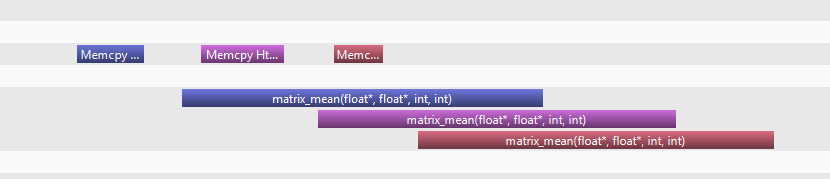
\includegraphics[width=\linewidth]{images/overlap_calcolo_media.PNG}
	\caption{Gli stream per il calcolo della media}
	\label{fig:means}
\end{figure}

\paragraph{Media totale}
La media totale � calcolata con il kernel \textbf{\textit{add\_vectors}} che esegue la somma degli C-vettori risultati dal calcolo precedente e utilizzando il kernel \textbf{\textit{div\_by\_scalar}} che esegue la divisione del vettore per uno scalare che � pari al numero di classi.\\
Naturalmente il vettore media totale avr� dimensione 1xM.
 
\subsection{Between-scatter matrix}
Il calcolo della Between-scatter matrix necessita di tre kernel.\\
Il kernel \textbf{\textit{diff\_vect}} si occupa di calcolare la differenza tra due vettori di dimensione \textit{M}, nel caso specifico tra il vettore media locale i-esimo e media globale. Il kernel viene lanciato su un numero di thread pari alla dimensione dei vettori suddivisi su pi� blocchi.\\
Successivamente viene eseguito il kernel \textbf{\textit{vector\_prod}} per il calcolo del prodotto tra il vettore in uscita dal kernel precedente e la sua trasposta. Il risultato � una matrice quadrata di dimensione \textit{M X M}.\\
L'ultimo punto � la somma di tutte le C matrici in uscita dal kernel precedente ed � eseguito dal kernel \textbf{\textit{add\_matrix}}.\\
Per ogni classe viene eseguito il gruppo dei tre kernel sopra descritti in stream diversi per permettere un livello di esecuzione concorrente maggiore in caso di dimensione del dataset ridotto.

\subsection{Within-scatter matrix}
Il calcolo della Within-scatter matrix si avvale di cinque kernel qui sotto descritti.\\
\begin{itemize}
	\item \textbf{\textit{diff\_matr\_vect}}: � il kernel che si occupa di sottrarre il vettore media della classe i-esima dalla i-esima matrice, riga per riga.
	\item \textbf{\textit{transposeSmem}}: esegue la trasposizione della matrice in ingresso
	\item \textbf{\textit{mat\_prod\_shared}} si occupa di eseguire il prodotto tra matrice i-esima trasposta e la stessa matrice non trasposta.
	\item  \textbf{\textit{div\_by\_scalar}}: esegue la divisione della matrice in ingresso per uno scalare.
	\item \textbf{\textit{add\_matrix}}: esegue la delle matrici risultati dalle operazioni precedenti delle C-classi
\end{itemize}
Essendo piccoli kernel, l'utilizzo di stream pari al numero di matrici mi ha permesso di ottenere un overlapping tra i kernel appartenenti a stream diversi come mostrato in figura \ref{fig:overlapprodotto}
\begin{figure}
	\centering
	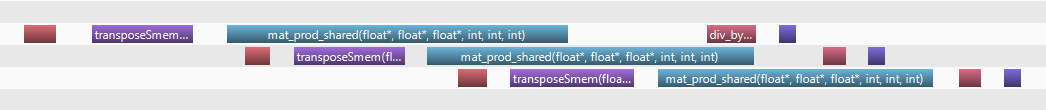
\includegraphics[width=0.7\linewidth]{images/overlap_prodotto}
	\caption{overlapping computazionale}
	\label{fig:overlapprodotto}
\end{figure}


\subsection{Calcolo matrice inversa di SW}
Per il calcolo della matrice inversa ho utilizzato le funzioni \textit{cublasSgetrfBatched()} e \textit{cublasSgetriBatched()} della libreria cuBLAS che eseguono la fattorizzazione LU. Successivamente al calcolo ho eseguito il prodotto tra la matrice inversa ottenuta e la matrice SB, tramite il kernel \textbf{\textit{matrix\_prod}}

\subsection{Calcolo autovalori e autovettori}
Per il calcolo degli autovalori e degli autovettori ho utilizzato la funzione \textit{cusolverDnDsyevd} della libreria cuSOLVER che esegue la Singular Value Decomposition per il calcolo degli autovettori e degli autovalori della matrice quadrata in ingresso \(Mat^{MxM}\)

\subsection{Calcolo dei nuovi dati}
Una volta ottenuto autovettori e rispettivi autovalori al passo precedente, ho selezionato gli C-1 autovettori che hanno gli autovalori massimi.\\
Ho quindi moltiplicato la matrice originale, e.g. nel caso di 4096 campioni \(Mat^{4094x128}\) per questi C-1 autovettori tramite il kernel \textbf{\textit{mat\_prod\_shared}} ottenendo cos� la nuova proiezione. La nuova matrice avr� quindi dimensione \(Mat^{4096x(C-1)}\)\\
Ho utilizzato un numero di stream pari al numeri di matrici e \textit{cudaMemcpyAsync} per sovrapporre la computazione del kernel che calcola il prodotto matriciale e la copia dei dati dalla device memory alla host memory per poter successivamente eseguire il plot a video.

\subsection{Plotting}
Per la presentazione del grafico ho utilizzato \textbf{Gnuplot} in tutti e due gli algoritmi.\\
In figura \ref{fig:plottingdata} � mostrato un grafico dei dati rispetto alle prime due componenti. In alto sono proiettati i dati originali mentre nell'area in basso i dati trasformati.

\begin{figure}[H]
	\centering
	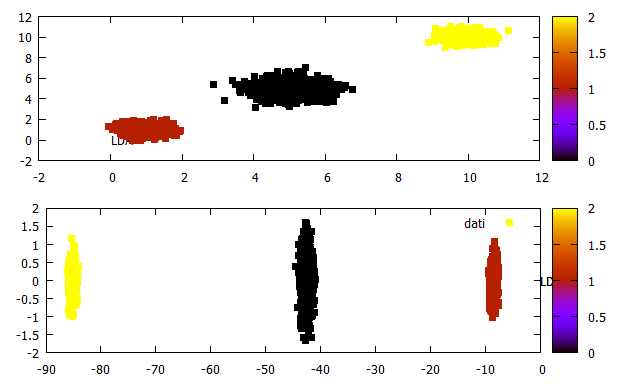
\includegraphics[width=0.7\linewidth]{images/plotting_data}
	\caption{originale e nuova proiezione}
	\label{fig:plottingdata}
\end{figure}


\section{Simulazione ed esperimenti}
Oltre all'algoritmo parallelo presentato qui nella sezione precedente, ho sviluppato anche un algoritmo per LDA sequenziale per verificare l'effettivo speed-up raggiunto dal primo rispetto al secondo.
\subsection{Dataset}
Per il benchmark ho utilizzato un dataset generato con una distribuzione normale multivariata. Ogni classe � costituita da 128 feature per campione ed un totale di 4096 istanze per classe.\\
In termini matematici, ogni classe � rappresentata da una matrice \(Mat^{4096 X 128}\).
\subsection{Risultati ottenuti}
Il software � stato eseguito su un computer con le seguenti caratteristiche:
\begin{itemize}
	\item GPU: NVIDIA GeForce 610M, compute capability  2.1, architettura FERMI (2.1) con 48 Cores/SM.
	\item CPU: Intel(R) Core(TM) i7-3630QM CPU @ 2.40GHz, 2401 Mhz, 4 core, 8 processori logici
\end{itemize}
Ho eseguito il calcolo del tempo impiegato dall'algoritmo tenendo fissato il numero di classi e di feature e variando il numero di campioni incrementandolo come potenza di due fino al raggiungere il valore massimo del dataset.\\
Per ogni step, ho eseguito l'algoritmo dieci volte ed elaborato la media dei tempi misurati per cercare di minimizzare l'effetto di eventuali outlier.\\\\
In figura \ref{fig:speedup} � mostrato il grafico dello speed-up della versione parallela rispetto all'implementazine classica. Come � possibile notare, minore � il carico, cio� il numero di osservazioni che l'algoritmo deve elaborare e minore � la differenza prestazionale tra le due versioni. All'aumentare delle osservazioni, a parit� di numero di feature, lo speedup aumenta.
\begin{figure}[H]
	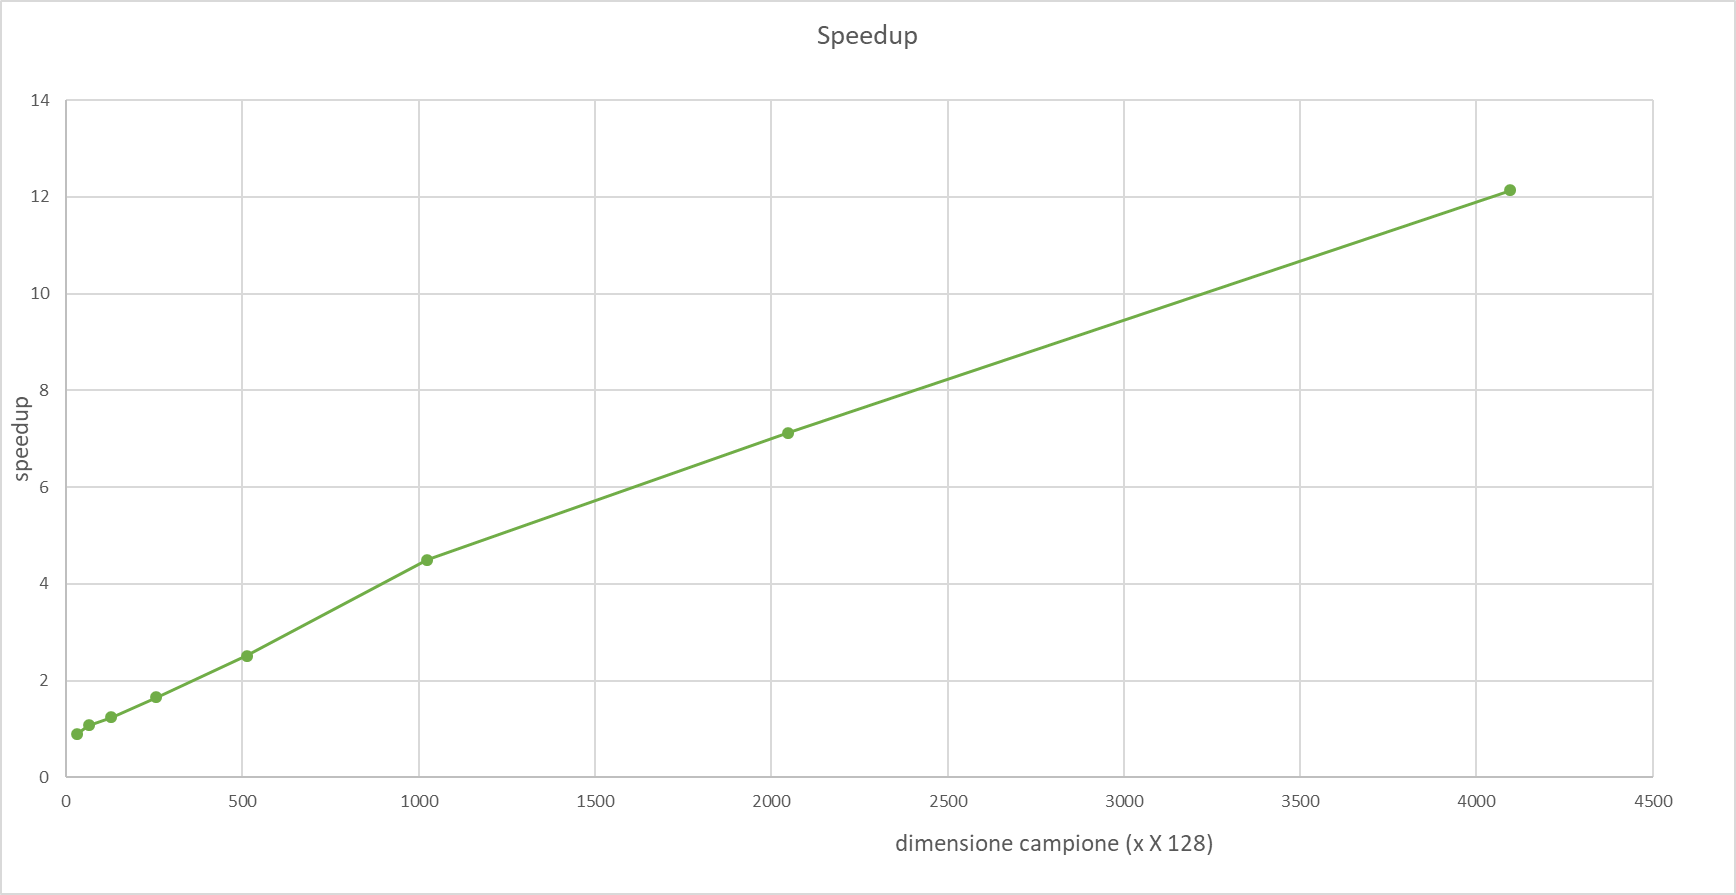
\includegraphics[width=\linewidth]{images/speedup.png}
 	\caption{Speed-up}
 	\label{fig:speedup}
\end{figure}

La figura \ref{fig:ratio} mostra i tempi impiegati dai due algoritmi dove la versione parallela � rappresentata da una quasi-retta orizzontale, mentre la versione sequenziale da una retta inclinata che mostra come aumentano i tempi di calcolo all'aumentare del numero di osservazioni. 
\begin{figure}[H]
	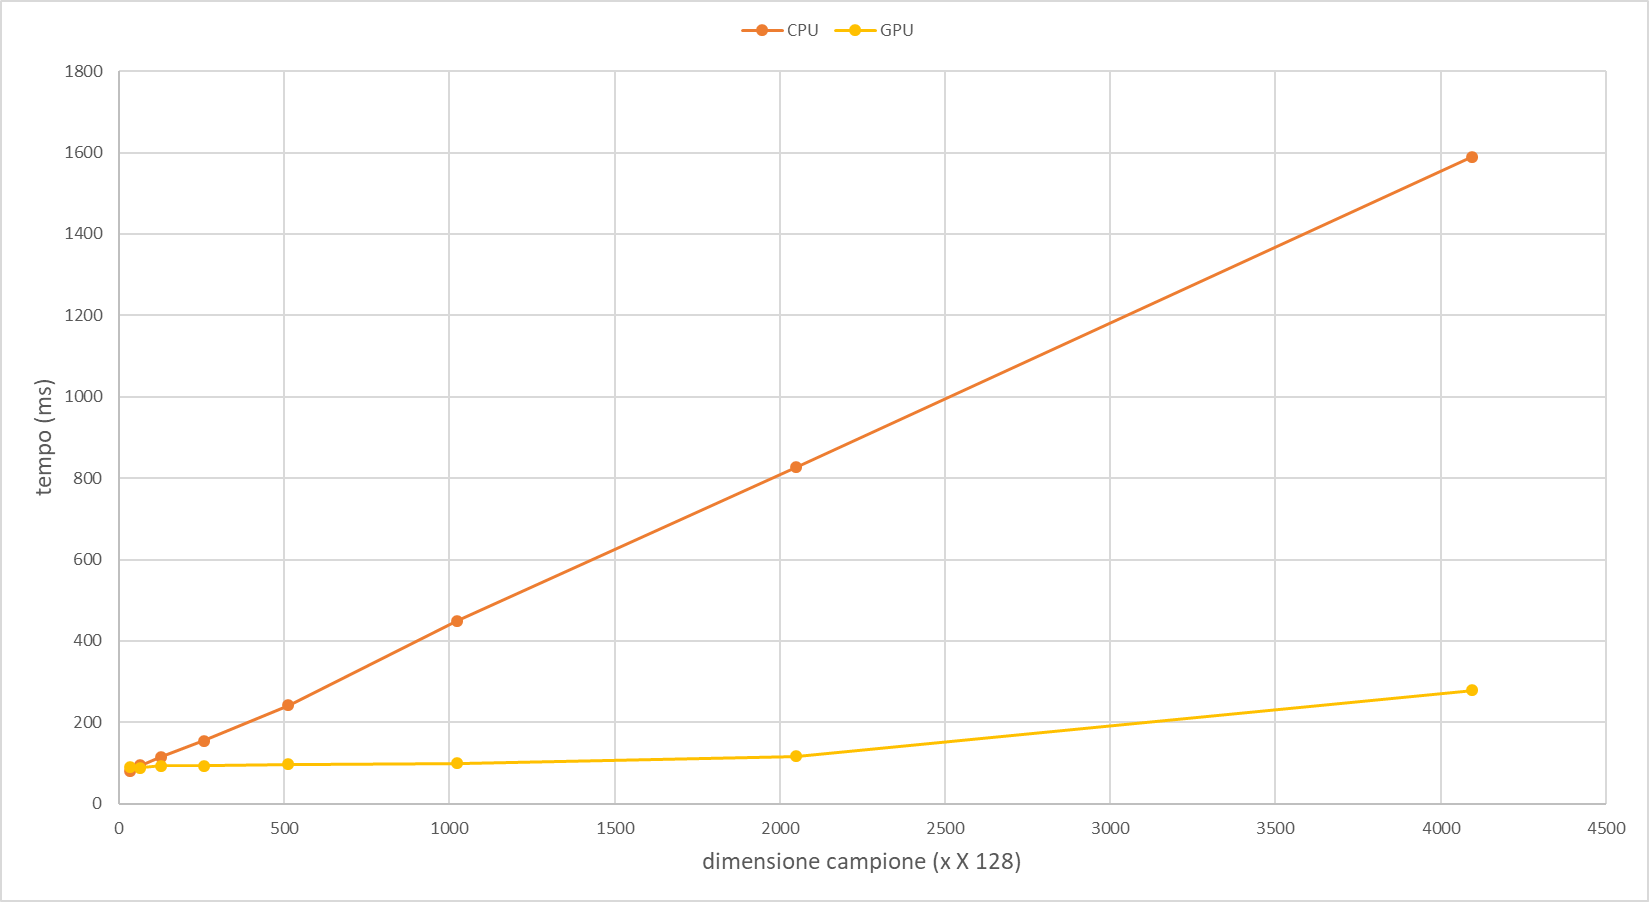
\includegraphics[width=\linewidth]{images/ratio.png}
	\caption{tempi}
	\label{fig:ratio}
\end{figure}

\end{document}